\section{Graph Theory}
This section describe the interconnected components in the water distributed network (WDN) using a concept called Graph Theory.

\subsection{The incident matrix}
When using graph theory as an analytical tool the incident matrix $H$ comes in handy when describing the connection between edges and nodes. The rules shown below has been used as guidelines when writing up the incident matrix for a graph network. 

\begin{equation*}
H_{i,j} = \begin{cases}
    -1 & \text{If the $j^{th}$ edge enters the $i^{th}$ node} \\
    0 & \text{If the $j^{th}$ edge is not connected to the $i^{th}$ node} \\
    1 & \text{If the $j^{th}$ edge s leaving the $i^{th}$ node}
\end{cases}
\end{equation*} %Description of the incident matrix

\begin{figure}[h!]
    \centering
    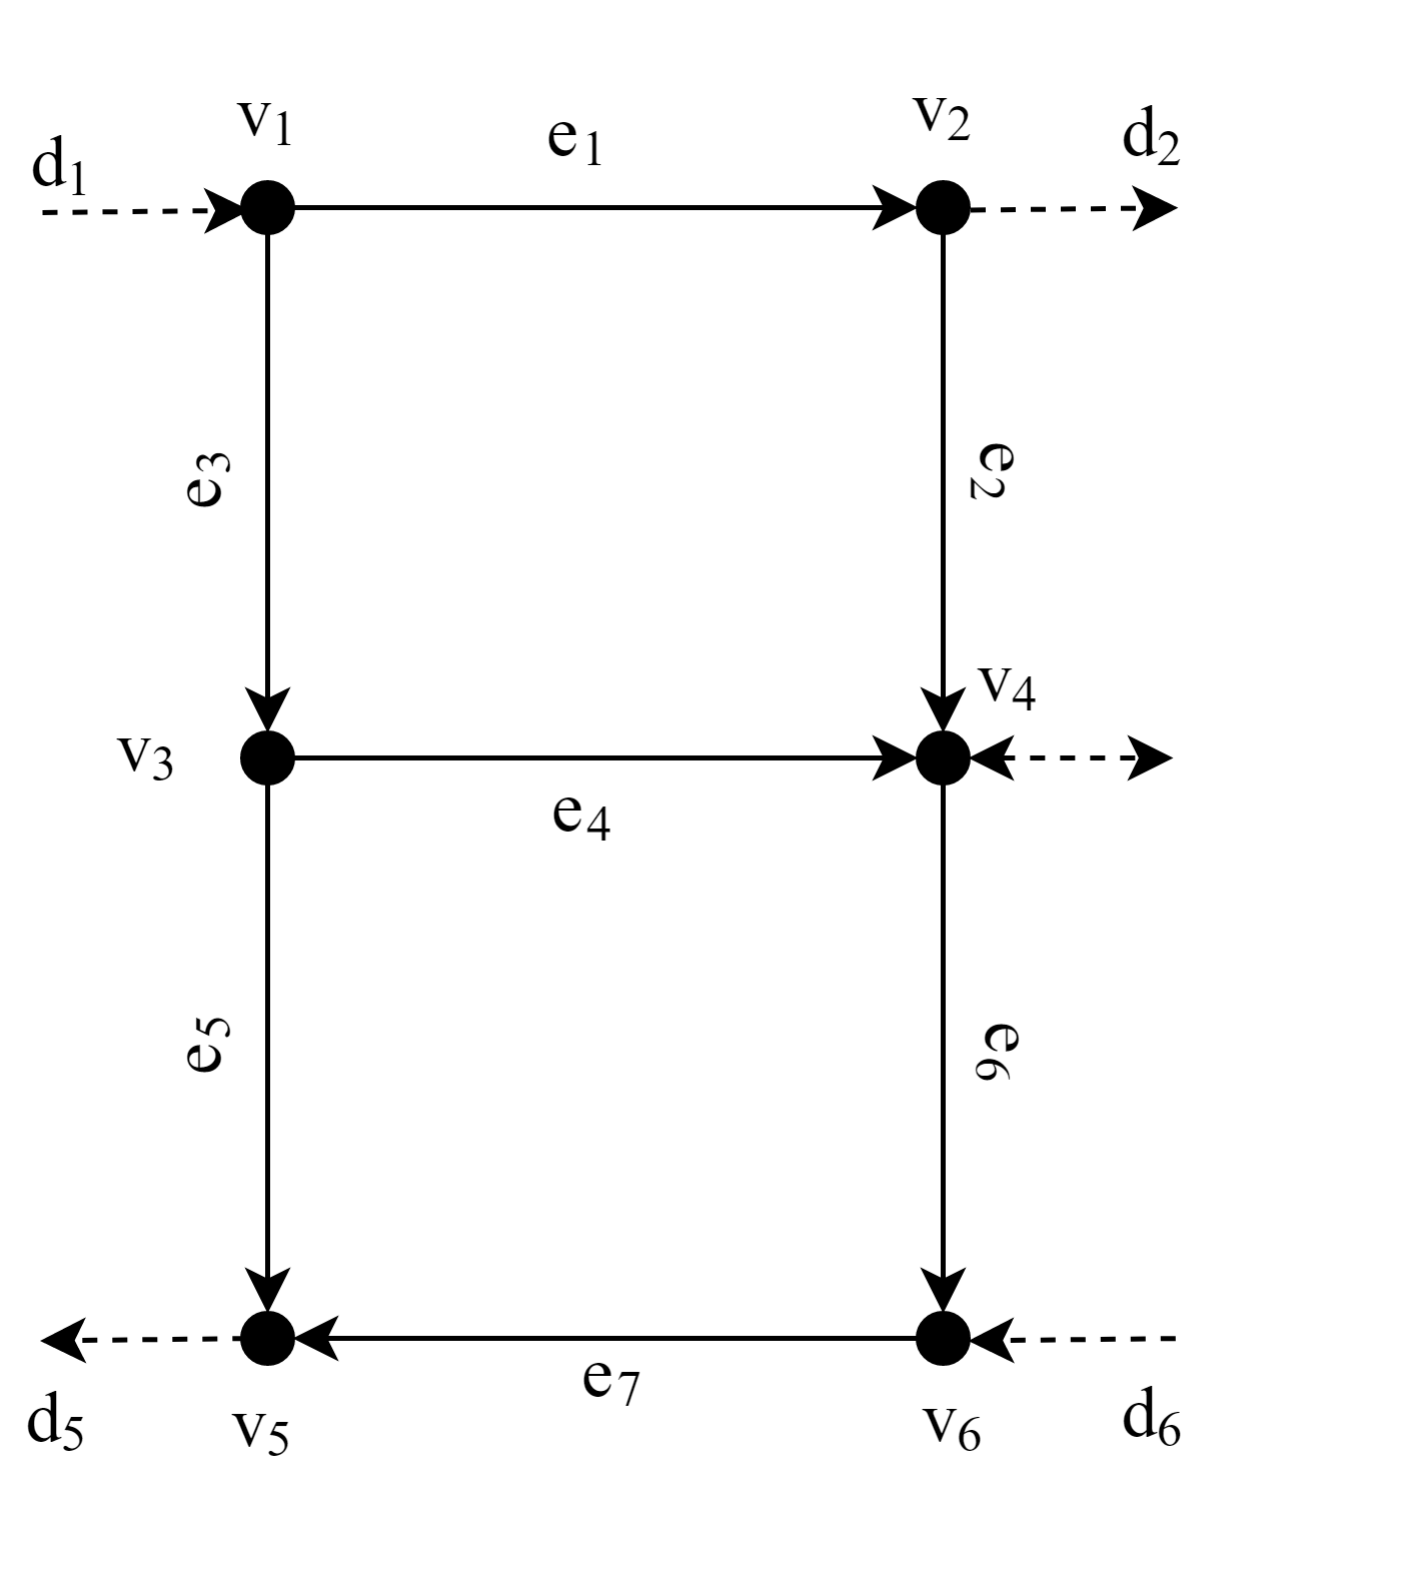
\includegraphics[width=0.5\textwidth]{MathiasTest/Pictures/Graph.png}
    \caption{Graph of simplified WDN network \cite{}}
    \label{fig:Graph
    }
\end{figure}

When applying the rules shown above for the simplified graph model of the WDN the incident matrix in \eqref{eq:H_simplified}.
\begin{equation}
    H = \begin{bmatrix}
1 & 0 & 1 & 0 & 0 & 0 & 0\\
-1 & 1 & 0 & 0 & 0 & 0 & 0\\
0 & 0 & -1 & 1 & 1 & 0 & 0\\
0 & -1 & 0 & -1 & 0 & 1 & 0\\
0 & 0 & 0 & 0 & -1 &  0  & -1\\
0 & 0 & 0 & 0 & 0 & -1 & 1
\end{bmatrix}
\label{eq:H_simplified}
\end{equation} %The incident matrix for system

The reduced incident matrix by taking an arbitrary vertex as a reference, and removing that vertex-row from \eqref{eq:H_simplified}. We chose the $4^{th}$ vertex, which results in the following reduced incident matrix:
\begin{equation}
    \bar{H} = \begin{bmatrix}
1 & 0 & 1 & 0 & 0 & 0 & 0\\
-1 & 1 & 0 & 0 & 0 & 0 & 0\\
0 & 0 & -1 & 1 & 1 & 0 & 0\\
0 & 0 & 0 & 0 & -1 &  0  & -1\\
0 & 0 & 0 & 0 & 0 & -1 & 1
\end{bmatrix}
\end{equation}

\subsection{The loop matrix}

The loop-matrix can be calculated in one of two ways. The first one is shown in the equation below

\begin{equation}
    B = \begin{bmatrix}
I & -\bar{H}_{C}^{T}\cdot\bar{H}_{T}^{-T}
\end{bmatrix}
\end{equation}

With $H_{c}$ and $H_{T}$ being the cord and tree component of the reduced incident matrix.